\documentclass[aspectratio=169]{beamer}

\usepackage{tikzlings}
\setbeamertemplate{navigation symbols}{}
\graphicspath{{include/}}

% trick taken from https://topanswers.xyz/tex?q=1989
\tikzset{
    use page relative coordinates/.style={
        shift={(current page.south west)},
        x={(current page.south east)},
        y={(current page.north west)}
    },
}

\begin{document}

\begin{frame}
  \begin{tikzpicture}[remember picture, overlay]

    \node at (9,0) {\includegraphics[width=10cm]{Firenze_aka_Florence,_Italy_(42195612411)}};

    \node[xshift=2cm,xscale=-1] at (2+\insertoverlaynumber*8/350,1) {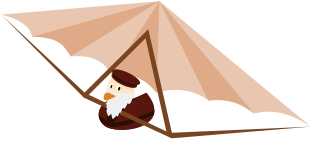
\includegraphics[width=2.5cm]{Hang_gliding_leonardo}};

    \fill[xshift=2cm,even odd rule,brown!20!darkgray!60!black,draw=brown!20!darkgray!80!black,line width=6pt]
      (current page.south west) rectangle (current page.north east) (3,-3) -- ++(2,0) -- ++(0,4.5) arc [start angle=0, end angle=180, radius=1] -- (3,-3)
      (5.5,-3) -- ++(2,0) -- ++(0,5) arc [start angle=0, end angle=180, radius=1] -- (5.5,-3)
      (8,-3) -- ++(2,0) -- ++(0,4.5) arc [start angle=0, end angle=180, radius=1] -- (8,-3)
      ;

    \node[draw=brown!20!darkgray!80!black,line width=6pt] at (2,0.5) {\includegraphics[width=3.5cm]{IMG_4528}};

    \node at (9,-1) {
\includegraphics[width=5cm]{dante_duck}};

    \fill[brown!60!black] (current page.south west) rectangle ++(\paperwidth,2.5cm);

    \fill[xshift=2cm,white!70!brown] (4.5,-4.6) -- ++(1.5,0) -- ++(-0.15,1.8) -- ++(-1.2,0) -- cycle;

    \draw[xshift=2cm,line width=0.7pt] (4.7,-4.3) -- ++(1,0);
    \draw[xshift=2cm,line width=0.7pt] (4.7,-4.1) -- ++(1,0);
    \draw[xshift=2cm,line width=0.7pt] (4.7,-3.9) -- ++(1,0);
    \draw[xshift=2cm,line width=0.7pt] (4.7,-3.7) -- ++(1,0);

    \begin{scope}[xshift=sin(2*\thepage)*0.5cm]
      \fill[xshift=2cm,white] (5.2,-3.5) ellipse [x radius=0.1,y radius=0.5];
      \draw[xshift=2cm,white,line width=1.5pt] (5.2,-3.5) -- ++(0,-0.7);
    \end{scope}

    % credit for background image
    \node[white,text width=\paperwidth,font=\tiny,align=center] at ([yshift=0.35cm]current page.south) {
      Image source: \url{https://commons.wikimedia.org/wiki/File:Firenze_aka_Florence,_Italy_(42195612411).jpg} (by Larry Lamsa, CC BY 2.0)
%      \linebreak Music source: Pierre Attaingnant -- Basse danse La Magdalena
    };

    \fill<350->[black,opacity=(\insertoverlaynumber-350)/10] (current page.south east) rectangle (current page.north west);

  \end{tikzpicture}
  \pause[360]
\end{frame}

\begin{frame}
\begin{tikzpicture}[remember picture,overlay]
  \fill[brown!60!black] (current page.south west) rectangle (current page.north east);
  \node at (current page.center) {\includegraphics[height=.9\paperheight]{parchment}};

   \fill<-10>[black,opacity=1-\insertoverlaynumber/10] (current page.south east) rectangle (current page.north west);
\end{tikzpicture}
\pause[175]
\end{frame}

\end{document}